% !TEX root = ../../../main.tex
% 来源：中学数学实验教材·第二册（几何）
% 章节：直线形 / 三角形
% 原始文件：3.tex，行 1293-1301
% 类型：tikz
% ---
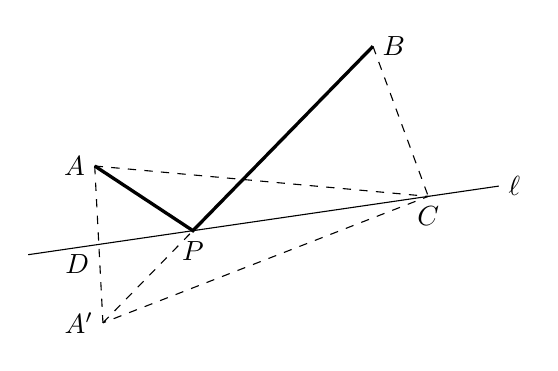
\begin{tikzpicture}[xscale=.6, rotate=5]
\draw (-2,0)--(8,0)node[right]{$\ell$};
\draw[dashed](-.5,1)node[left]{$A$}--(-.5,-1)node[left]{$A'$};
\draw[dashed](-.5,-1)--(5.5,2)node[right]{$B$};
\draw[very thick](-.5,1)--(1.5,0)node[below]{$P$}--(5.5,2);
\node at (-.5,0)[below left]{$D$};
\draw[dashed](-.5,1)  -- (6.5,0) node[below]{$C$}--(-.5,-1);
\draw[dashed](5.5,2)  -- (6.5,0);
\end{tikzpicture}
